\documentclass[a4paper]{report}
\usepackage[utf8]{inputenc}
\usepackage{amssymb}
\usepackage{amsmath}
\usepackage[margin=1in]{geometry}
\usepackage{graphicx}
\usepackage{verbatim}
\usepackage{bm}
\usepackage{listings}

\lstset{
  basicstyle=\ttfamily,
  mathescape
}

\title{Models - Notes}
\author{André Oskar Andersen}
\date{}

\begin{document}
    
\maketitle

\chapter*{Mask R-CNN}
\section*{Abstract}
Our approach efficiently detects objects in an image while simultaneously generating a high-quality segmentation mask for each instance. 

\section*{1. Introduction}
Instance segmentation is challenging because it requires the correct detection of all objects in an image while also precisely segmenting each instance. It therefore combines elements from the classical computer vision tasks of object detection, where the goal is to classify individual objects and localize each using a bounding box, and semantic segmentation, where the goal is to classify each pixel into a fixed set of categories without differentiating object instances (we use \textit{object detection} to denote detection via \textit{bounding boxes}, not masks, and \textit{semantic segmentation} to denote per-pixel classification without differentiating instances. Yet we note that \textit{instance segmentation} is both semantic and a form of detection).
\\
\\
We found it essential to decouple mask and class prediction: we predict a binary mask for each class independently, without competition among classes, and rely on the network's RoI classification branch to predict the category.
\\
\\
Finally, we showcase the generality of our framework via the task of human pose estimation on the COCO keypoint dataset. By viewing each keypoint as a one-hot binary mask, with minimal modification Mask R-CNN can be applied to detect instance--specific poses.

\section*{3. Mask R-CNN}
We behin by briefly reviewing the Faster R-CNN detector. Faster R-CNN consists of two stages. The first stage, called Region Proposal Network (RPN), proposes candidate object bounding boxes. The second stage, which is in essence Fast R-CNN, extracts features using RoIPool from each candidate box and performs classifcation and bounding-box regression. 
\\
\\
Mask R-CNN adopts the same two-stage procedure, with an identical first stage (which is RPN). In the second stage, in parallel to predicting the class and box offset, Mask R-CNN also outputs a binary mask for each RoI. This is in contrast to most recent systems, where classification depends on mask predictions. Our approach follows the spirit of Fast R-CNN that applies bounding-box classification and regression in parallel (which turned out to largely simplify the multi-stage pipeline or original R-CNN).
\\
Formally, during training, we define a multi-task loss on each sampled RoI as $L = L_{cls} + L_{box} + L_{mask}$. The classification loss $L_{cls}$ and bounding-box loss $L_{box}$ are identical as those defined in the Fast R-CNN paper. The mask branch has a $Km^2$-dimensional output for each RoI, which encodes $K$ binary masks of resolution $m \times m$, one for each of the $K$ classes. To this we apply a per-pixel sigmoid, and efine $L_{mask}$ as the average binary cross-entropy loss. For an RoI associated with ground-truth class $k$, $L_{mask}$ is only defined on the $k$-th mask (other mask outputs do not contribute to the loss).
\\
Our definition of $L_{mask}$ allows the network to generate masks for every class without competition among classes; we rely on the dedicated classifcation branch to predict the class label used to select the output mask. This decouples mask and class prediction.
\\
\\
\textbf{Mask Representation}: Specifically, we predict an $m \times m$ mask fro meach RoI using an FCN (fully convolutional network). This allows each layer in the mask branch to maintain the explicit $m \times m$ object spatial layout spatial dimensions. Unlike previous methods that resort to $fc$ layers for mask prediction, our fully convolutional representation requires fewer parameters, and is more accurate as demonstrated by experiments.
\\
\\
This pixel-to-pixel behavior requires our RoI features, which themselves are small feature maps, to be well aligned to faithfully preserve the explicit per-pixel spatial correspondence. This motvaited us to develop the following \textit{RoIAlign} layer that plays a key role in mask prediction.
\\
\\
\textbf{RoIAlign}: RoIPool is a standard operation for extracting a small feature map (e.g., $7 \times 7$) from each RoI. The quantization used by these operations introduce misalignments between the RoI and the extracted features. While this may not impact classification, it has a large negative effect on predicting pixel-accurate masks.
\\
To address this, we propose an RoIAlign layer that removes the harsh quantization of RoIPool, properly aligning the extracted fgeatures with the input. RoIAlign leads to large improvements.
\\
\\
\textbf{Network Architecture}: To demonstrate the generality of our approach, we instantiate Mask R-CNN with multiple architectures.

\section*{5. Mask R-CNN for Human Pose Estimation}
Our framework can easily be extended to human pose estimation. We model a keypoint's location as a one-hot mask and adopt mask R-CNN to predict $K$ masks, one for each of $K$ keypoint types.
\\
\\
\textbf{Implementation Details}: We make minor modifications to the se gmentation system when adapting it for keypoints. For each of the $K$ keypoints of an instance, the training target is a one-hot $m \times m$ binary mask where only a single pixel is labeled as foreground. During training, for each visible ground-truth keypoint, we minimize the cross-entropy loss over an $m^2$-way softmax output. We note that as in instance segmentation, the $K$ keypoints are still ttreated independently.


\chapter*{Understanding Mask R-CNN Basic Architecture}
\begin{figure}[h]
    \centering
    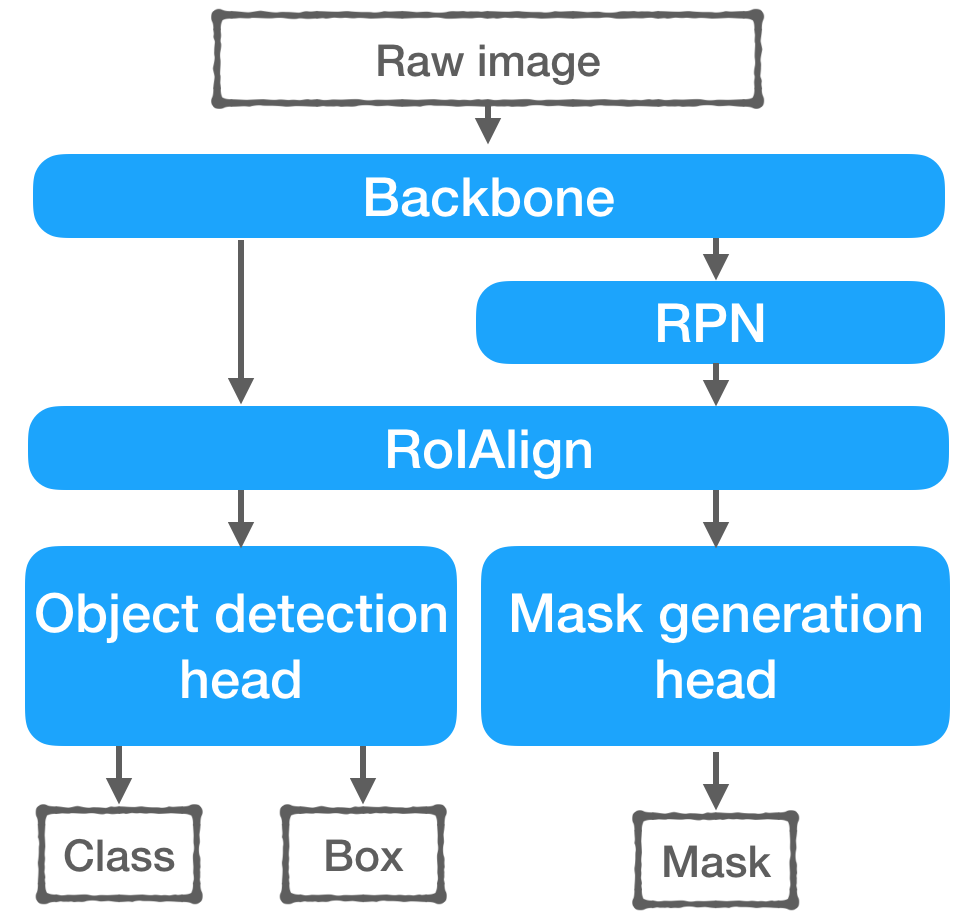
\includegraphics[width=0.4 \textwidth]{./entities/maskrcnn-big-picture.png}
    \caption{Overall Mask R-CNN architecture}
    \label{fig:RCNN_overall}
\end{figure}
Mask R-CNN is a popular deep learning framework for instance segmentation task in computer vision field. It adds fully convolutional networks (FCN) to Faster R-CNN to generate mask for each object.
\\
\\
Mask R-CNN can be composed by these parts: a backbone, a Region Proposal Network (RPN), a Region of Interest alignment layer (RoIAlign), a bounding-box object detection head and a mask generation head. The ove rall structure can be illustrated as in Figure \ref{fig:RCNN_overall}

\section*{1. Backbone}
\begin{figure}[h]
    \centering
    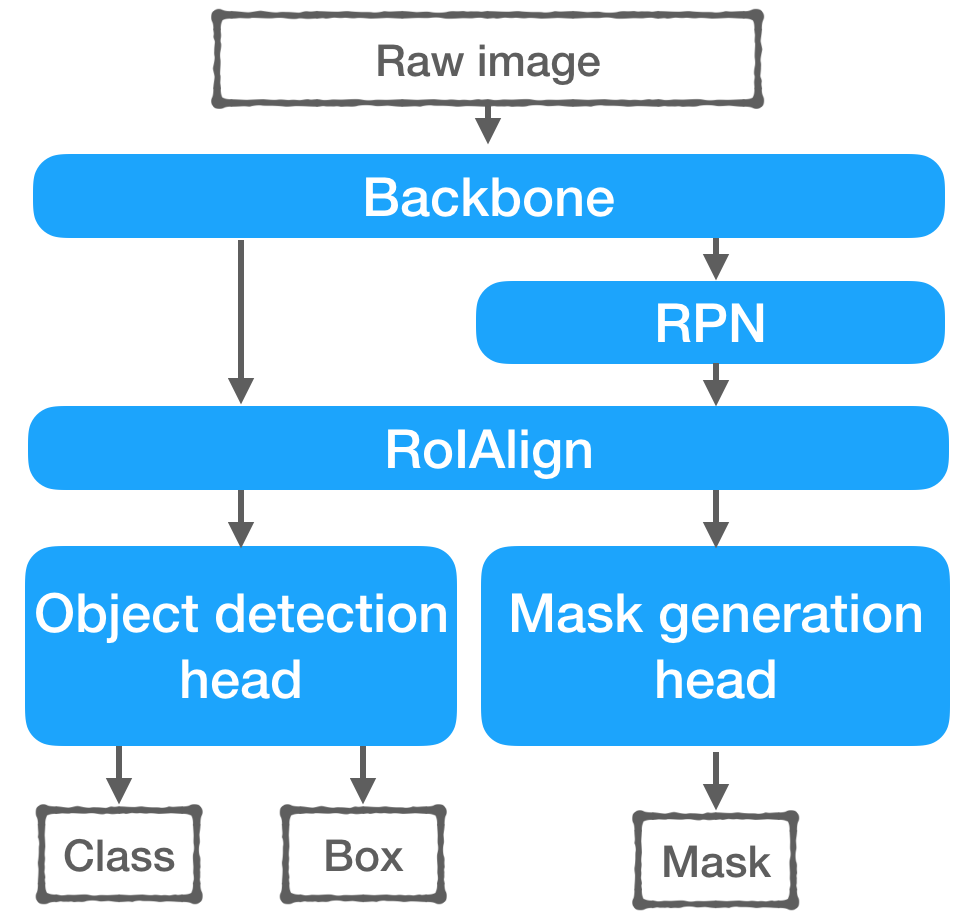
\includegraphics[width=0.4 \textwidth]{./entities/maskrcnn-big-picture.png}
    \caption{Mask R-CNN backbone}
    \label{fig:RCNN_backbone}
\end{figure}
A backbone is the main feature extractor of Mask R-CNN. When we feed a raw image into a backbone, data goes through blocks and turns into a feature map.
\\
\\
Feature map from the final convolutional layer of the backbone contains abstract informations of an image, e.g., different object instances, their classes and spatial properties. It is then fed to the RPN.

\section*{2. RPN}
\begin{figure}[h]
    \centering
    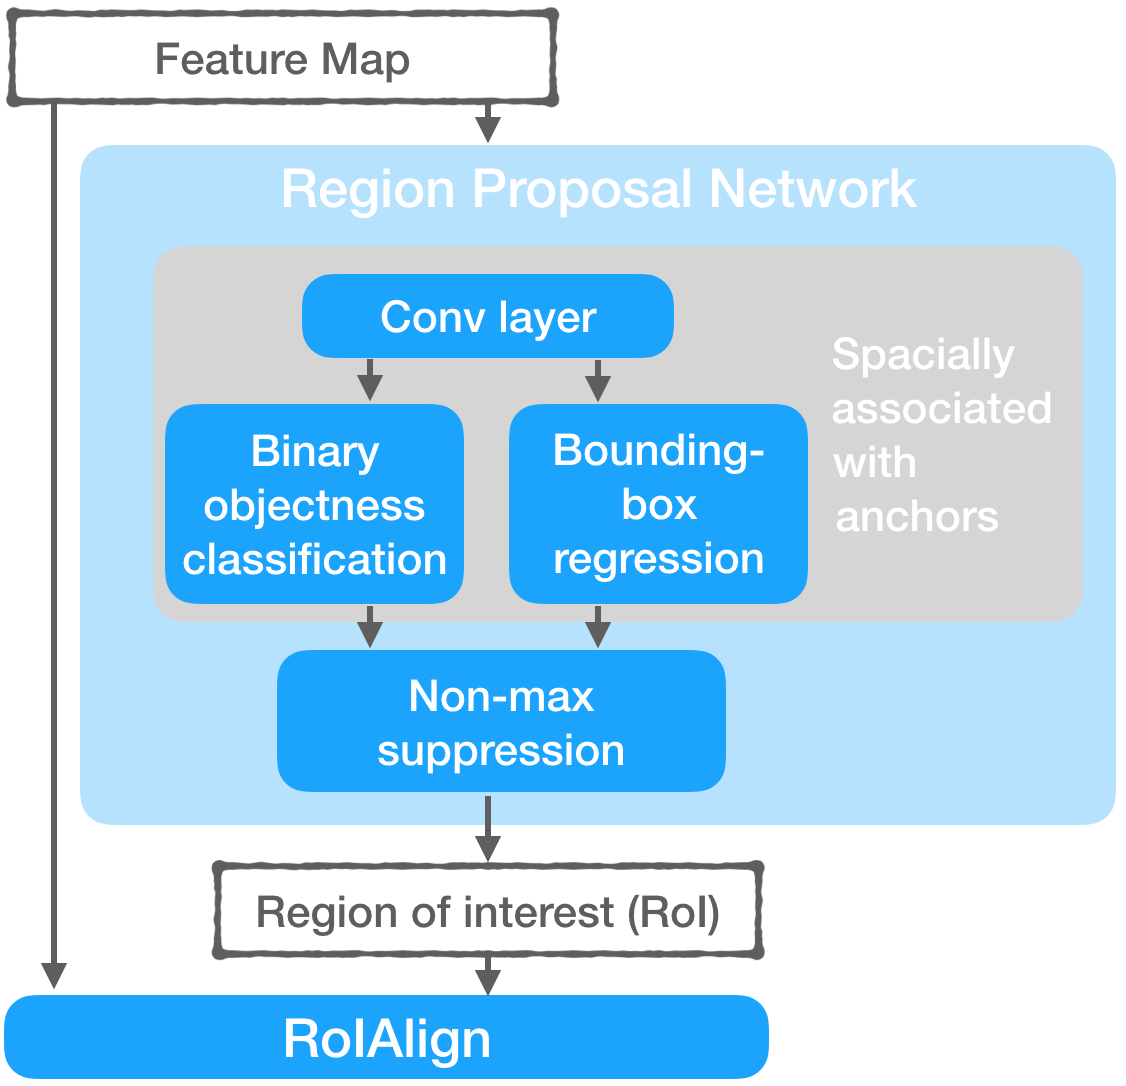
\includegraphics[width=0.4 \textwidth]{./entities/maskrcnn-rpn.png}
    \caption{Mask R-CNN RPN}
    \label{fig:RCNN_RPN}
\end{figure}
The function of RPN is to scan the feature map and propose regions that may have objects in them (Region of Interest or RoI). As so, we get a bunch of proposed RoIs. The next step is to find where exactly each RoI is in the feature map. It's called RoIAlign.

\section*{3. RoIAlign}
\begin{figure}[h]
    \centering
    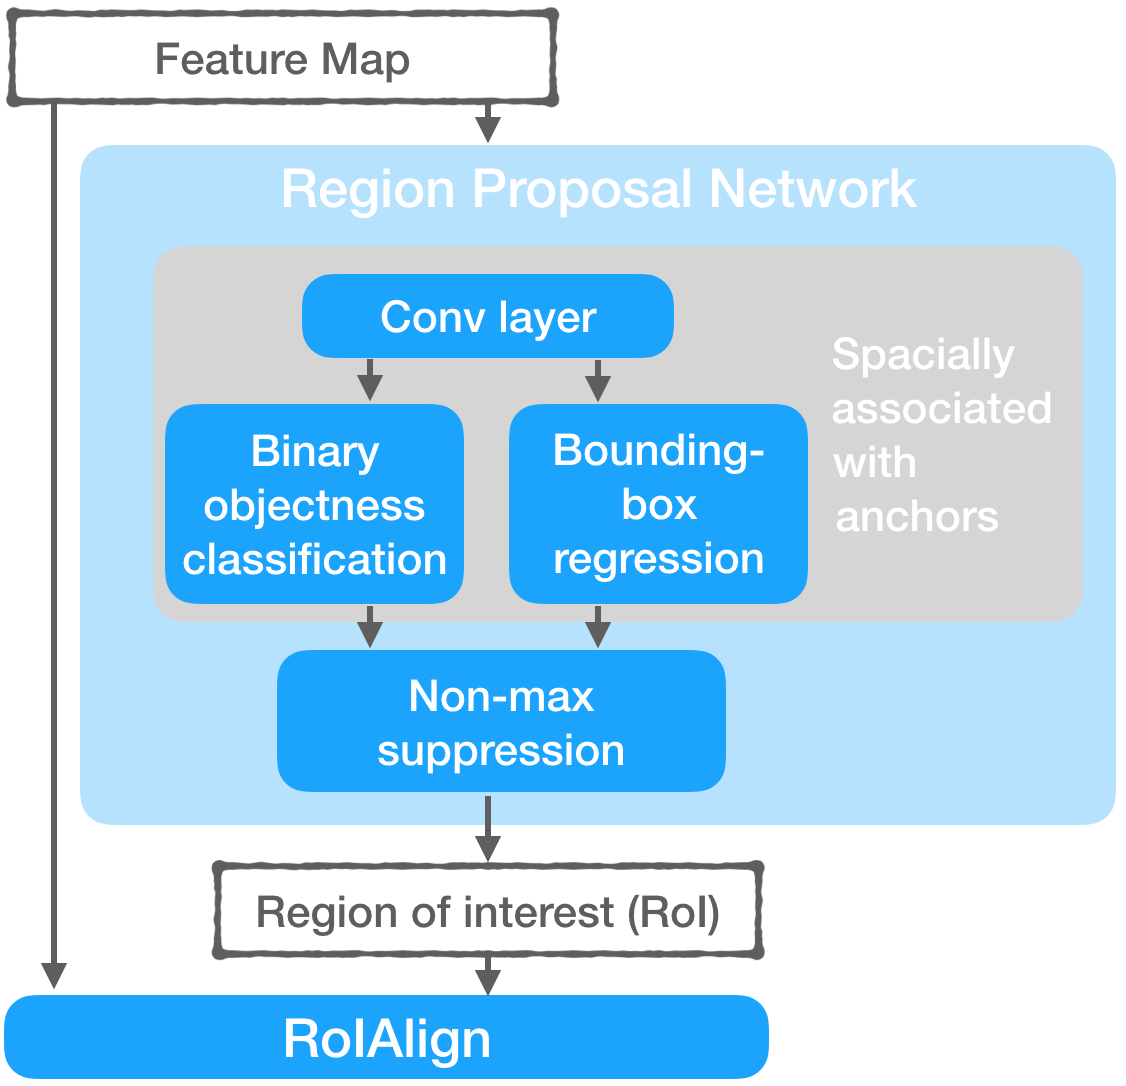
\includegraphics[width=0.4 \textwidth]{./entities/maskrcnn-rpn.png}
    \caption{Mask R-CNN RoIAlign}
    \label{fig:RCNN_RoIAlign}
\end{figure}
RoIAlign or Region of Interest alignment extracts feature vectors from a feature map based on RoI proposed by RPN, and turn them into a fix-sized tensor for further processes. The results represent every RoI's finer feature map and will be processed by two following parallel branches: object detection branch and mask generation branch.

\section*{4. Object detection branch}
\begin{figure}[h]
    \centering
    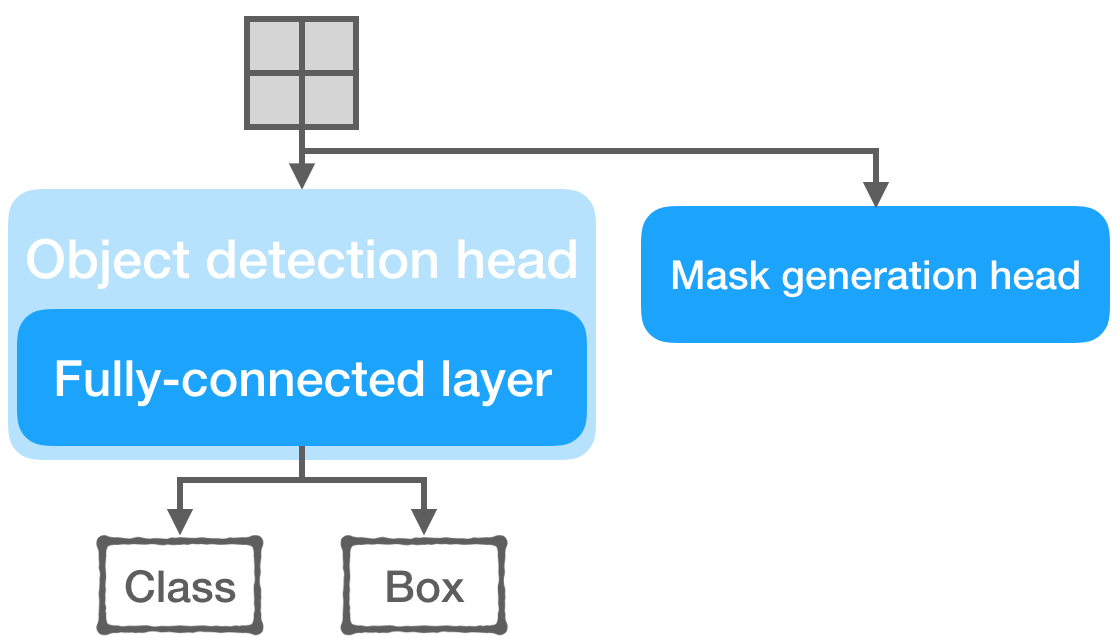
\includegraphics[width=0.4 \textwidth]{./entities/maskrcnn-object-detection-head.png}
    \caption{Mask R-CNN Object Detection Branch}
    \label{fig:RCNN_ODB}
\end{figure}
After we get individual RoI feature map, we can predict its object category and a finer instance bounding-box. This branch is a fully-connected layer that maps feature vectors to the final n classes and 4n instance bounding-box coordinates

\section*{5. Mask Generation Branch}
\begin{figure}[h]
    \centering
    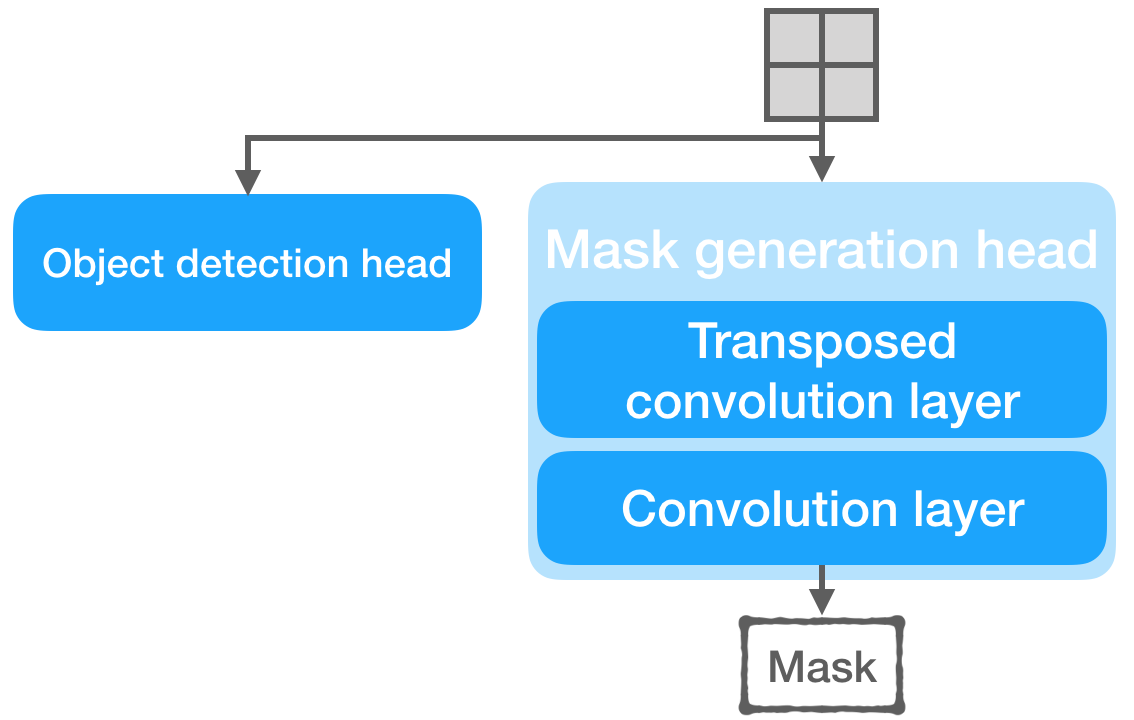
\includegraphics[width=0.4 \textwidth]{./entities/maskrcnn-mask-head.png}
    \caption{Mask R-CNN Mask Generation Branch}
    \label{fig:RCNN_MGB}
\end{figure}
On the mask generation branch, we feed RoI feature map to a transposed convolutional layer and a convolutional layer successively. This branch is a fully convolutional network. One binary segmentation mask is generated for one class. Then we pick the output mask according to the class prediction in object detection branch. In this way, per-pixel's mask prediction can avoid competition between different classes.

\chapter*{UniPose: Unified Human Pose Estimation in Single Images and Videos}
\section*{Abstract}
Our method is extended to UniPose-LSTM for multi-frame processing and achieves state-of-the-art results for temporal pose estimation in video. 

\begin{figure}[h]
    \centering
    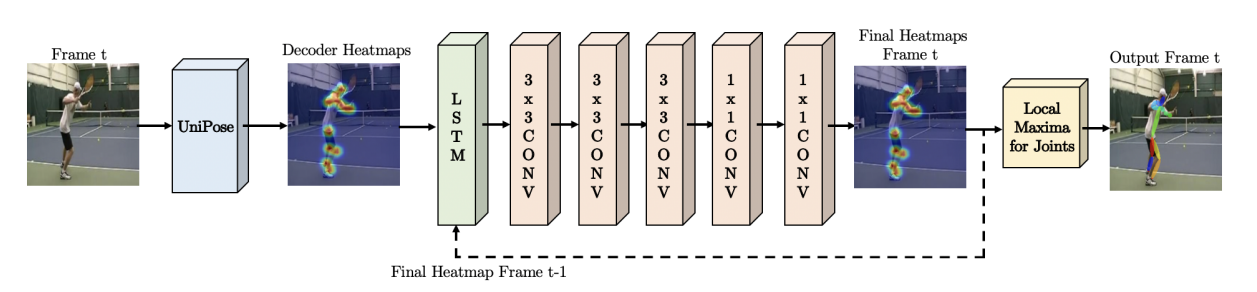
\includegraphics[width=0.8 \textwidth]{./entities/unipose.PNG}
    \caption{UniPose-LSTM architecture}
    \label{fig:Unipose}
\end{figure}
The UniPose architecture was modified to UniPose-LSTM for pose estimation in video. For video processing, it is useful to leverage the similarities and temporal correlation between consecutive frames.
\\
To operate in video processing mode, the UniPose architecture is augmented by an LSTM module that receives the final heatmaps from the previous frame along with the decoder heatmaps from the current frame. This network includes CNN layers following the LSTM to generate the final heatmaps used for joint detection.
\\
It was experimentally determined that accuracy impro ves when incorporating up to 5 frames in the LSTM, and a plateau in accuracy was observed for additional frames.

\section*{4. Datasets}
For video, two datasets are used: Penn Action and BBC Pose.
\\
Pen Action dataset contains 2,326 video sequences of 15 different activities including different sports, athletic acitivies, and playing instruments. The dataset was used to evaluate the performance of our architecture for temporal pose estimation and joint tracking.
\\
The BBC Pose dataset consists of 20 video from BBC. The BBC Pose dataset was utilized for the spcialized application of human pose for sign language.

\chapter*{LSTM Pose Machines}
\begin{figure}[h]
    \centering
    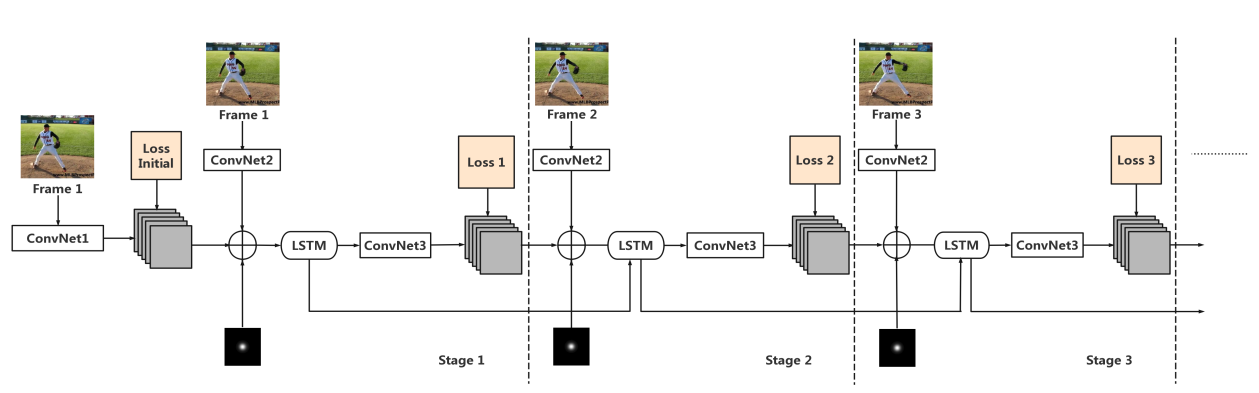
\includegraphics[width=0.8 \textwidth]{./entities/LSTM_pose_machine.PNG}
    \caption{Network architecture for LSTM Pose Machines}
    \label{fig:LSTM_pose_machine}
\end{figure}
\subsection*{3.2. LSTM Pose Machines}
\textbf{Details of the Model}.
Figure \ref{fig:LSTM_pose_machine} illustrates the structure for pose estimation on video.

\subsection*{4.1. Datasets}
JHMDB is a video-based dataset for pose estimation.




\end{document}